\documentclass{article}

% if you need to pass options to natbib, use, e.g.:
%     \PassOptionsToPackage{numbers, compress}{natbib}
% before loading neurips_2021

% ready for submission
\usepackage[final]{_report}

% to compile a preprint version, e.g., for submission to arXiv, add add the
% [preprint] option:
%     \usepackage[preprint]{_report}

% to compile a camera-ready version, add the [final] option, e.g.:
%     \usepackage[final]{_report}

% to avoid loading the natbib package, add option nonatbib:
%    \usepackage[nonatbib]{_report}

\usepackage[utf8]{inputenc} % allow utf-8 input
\usepackage[T1]{fontenc}    % use 8-bit T1 fonts
\usepackage{hyperref}       % hyperlinks
\usepackage{url}            % simple URL typesetting
\usepackage{booktabs}       % professional-quality tables
\usepackage{amsfonts}       % blackboard math symbols
\usepackage{nicefrac}       % compact symbols for 1/2, etc.
\usepackage{microtype}      % microtypography
\usepackage{xcolor}         % colors
\usepackage[pdftex]{graphicx}

\title{
  Kaggle - GettingStarted prediction Competition \\ 
  Digit Recognizer (MNIST)
}

% The \author macro works with any number of authors. There are two commands
% used to separate the names and addresses of multiple authors: \And and \AND.
%
% Using \And between authors leaves it to LaTeX to determine where to break the
% lines. Using \AND forces a line break at that point. So, if LaTeX puts 3 of 4
% authors names on the first line, and the last on the second line, try using
% \AND instead of \And before the third author name.

\author{%
  Steve Levesque \\
  \url{https://stevelevesque.dev} \\
  \texttt{hello@stevelevesque.dev}
}

\begin{document}

\maketitle

\begin{abstract}
  The digit recognition task in machine learning or data science is the "hello
  world" of the domain. It is a good point to start up in the field. This
  article will describe the steps used to achieve "acceptable" results (by this
  statement, a score around 99\%, and lower than 99.6\%), possible ways to 
  increase it fairly in terms of baises and cheating, and discard unreasonably
  high scores such as 99.957\% or worst like 100\%. The redaction's content 
  difficulty is made to be light and made for general public, for those who 
  could graspe that there are a lot of superficial explainations in term of
  results and advances.
\end{abstract}

\section{Introduction}
For this type of task, it is easily possible (especially as for today, 2021-22)
to build a model that can reach above 90\% in a matter of minutes, or around
97-99\% in less than an hour. The tricky part about MNIST digit recognition is
mainly for the last hundred digits or so, as for the model AND humans. Seeing
by ourselves such writings is hard even for us to classify since there are very
badly written number like a four that ressembles a lot to a nine and others of
the sort.

\section{MNIST Dataset}
\subsection{Data Description}
The MNIST dataset consists of numbers between 0 and 9 that are handwritten. The
traditionnal task with the digit is to classify each picture of 784 pixels or
of dimension $28 \times 28$ with 1 dimension of color (black and white) to its
rightful category (a number between 0 and 9 respectively).

\begin{figure}[!htbp]
  \centering
  \includegraphics[scale=0.5]{../plots/mnist_introduction_numbers.png}
  \caption{First 9 digits of the Kaggle MNIST test set}
\end{figure}


\subsection{Data Augmentation}
To help generalize in machine learning, it is a good solution to have more data
that is not the test set nor a subset/superset of it. (to avoid bias or at a
higher pitch, cheating) It is possible to modify the images of our train set
with small equivariant variations (invariant variations, as the word would
suggest, is just copying the image and doubling the size of our training set,
which is useless) such as translation, rotation and zooming (i.e. not as a 
whole 180 degrees, else 6 and 9 would be the same). \\

With the augmentations, digits will have more chances to be righfully classified
if someone writes with a more italic tone or with a unsteady pattern. We can see
in the first 9 digits of the test set of Figure 1 that there are four zeros
written with a different size, shape, marker size, etc.

\section{Algorithms}
\subsection{XGBoost}
"XGBoost is an optimized distributed gradient boosting library designed to be 
highly efficient, flexible and portable." The first sentence from their website
describes well XGBoost in a few words. It can train and predict with a score
quite acceptable for the little ammount of time it takes it to solve huge 
diverse problems.

The score is 93.78\% for about 10 minutes of training.

\subsection{KNN}
Another simple and easy algorithm to use is K Nearest Neighbors. It works well
with a lot of problems that takes distances into account. We can use the number
of neighbors equal to one to have a medium decent result. It won't be the best,
but with how MNIST is with distances towards each digit that are normally close
to eachother if they are of the same group, it will classify all even looking
numbers together without hassle. The score won't be 99\%, since there will be
errors when a seven looks like a one and all similar irregularities.

The score is 97.01\% for about 30 minutes of training.

\subsection{CNN}
However, CNN is of choice if the intent is to perform well on a task that
requires comupter vision such as this one. We start by defining a conv-net for
our model. Keras is used for the network, data augmenting, model saving/loading
and finally for prediction. Next, we choose the right number of epochs and batch
size for the training. When done, the final step is plotting and comparing the
results. It is important to see what is gain and for how much (i.e. time spent
for every 0.1\% gained).

\begin{figure}[!htbp]
  \centering
  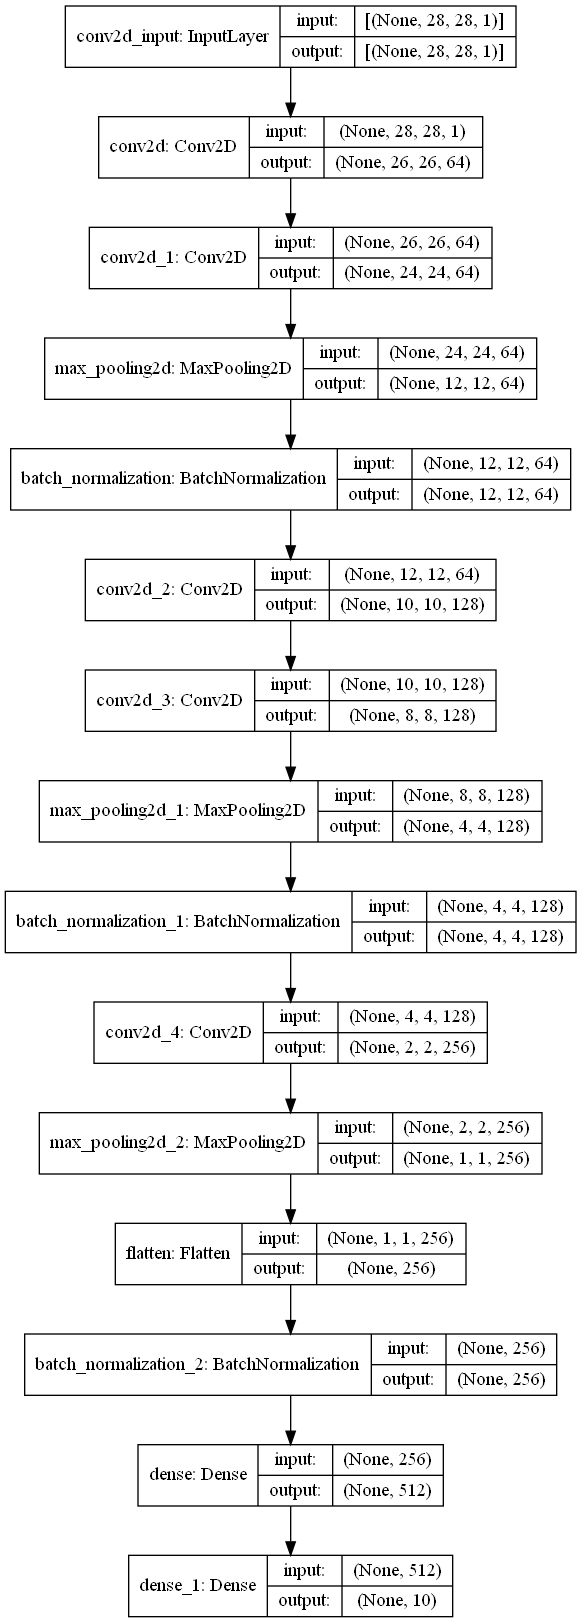
\includegraphics[scale=0.3]{../plots/mnist-supervised-classification-image-cnn_keras-model.png}
  \caption{Conv-net with Keras used for the model.}
\end{figure}

\begin{figure}[!htbp]
  \centering
  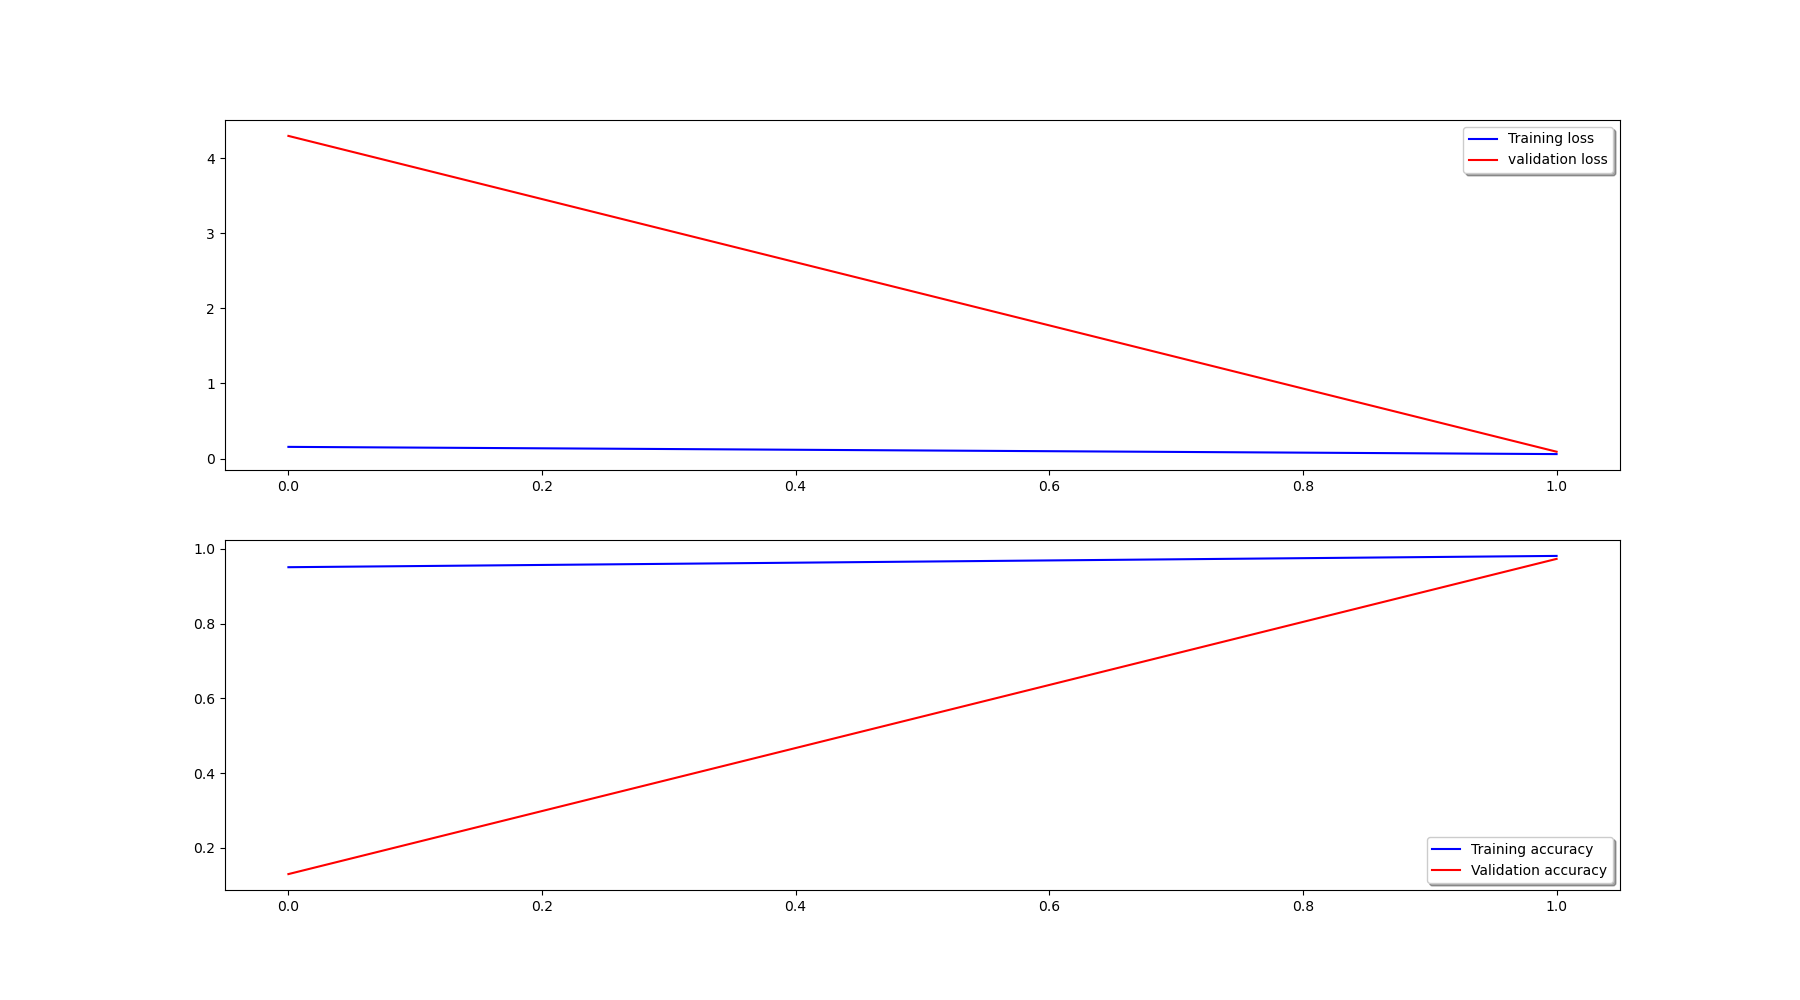
\includegraphics[scale=0.25]{../plots/mnist-supervised-classification-image-cnn_2epochs-128batch_curves.png}
  \includegraphics[scale=0.25]{../plots/mnist-supervised-classification-image-cnn_50epochs-64batch_curves.png}
  \caption{Loss and accuracy for 2-50 epochs and 128-64 respectively.}
\end{figure}

\begin{figure}[!htbp]
  \centering
  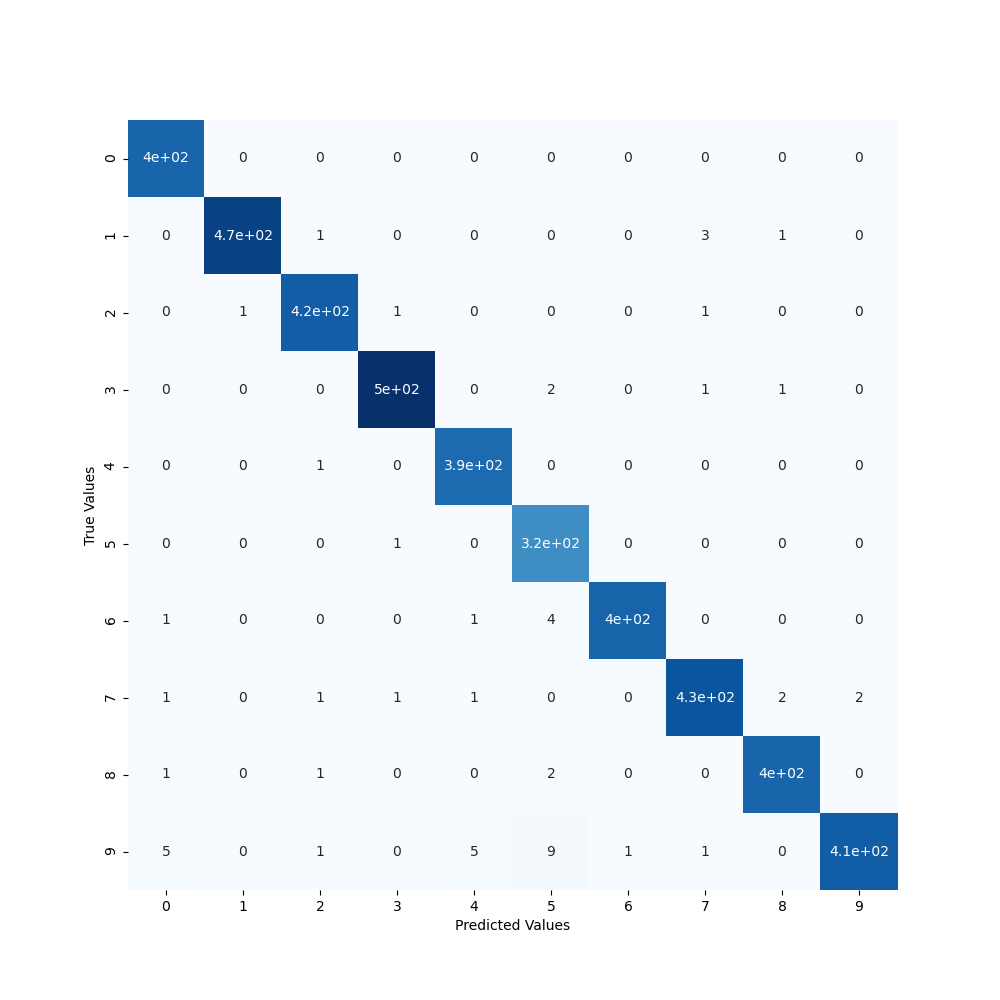
\includegraphics[scale=0.25]{../plots/mnist-supervised-classification-image-cnn_2epochs-128batch_confusion-matrix.png}
  \hspace{\fill}
  \includegraphics[scale=0.25]{../plots/mnist-supervised-classification-image-cnn_50epochs-64batch_confusion-matrix.png}
  \caption{Confusion matrix for 2-50 epochs and 128-64 respectively.}
\end{figure}

The results are made with data augmentation beforehand. With only 2 epochs and a
large batch size of 128, we can reach as high as 98.69\%. This is good taking
into account that it takes around 10 minutes to train. With 50 epochs and 64
batch size, we can reach up to 99.55\%. With double the ammount of epochs (100),
we only get 0.021\% increase. Thus around double the time for only that much
more.

The first score is (98.69\%) for about 10 minutes of training.

The second (99.55\%) for about 30 minutes of training.

The third (99.57\%) for about 1 hour of training.


\section{Results}
The table below contains results obtained from the algorithms above and some
other less legitimate techniques. Scores aboves 99.57\% will be discused on 
following sections. Above this treshold for the last digits more complicated to
classify, highter accuracy is always possible, but with high consumtion of time
and/or resources.

NB: The public score constitutes the private as well, since it is 100\% the data
for learning purposes.

\begin{table}[!htbp]
  \caption{Leaderboard Results by Algortihm}
  \label{results-table}
  \centering
  \begin{tabular}{lll}
    \toprule
    Algorithms     & Public   \\
    \midrule
    XGBoost & $\sim$93.78\% \\
    KNN (neighbours = 1) & $\sim$97.01\% \\
    CNN 2 epochs and 128 batch-size & $\sim$98.69\% \\
    CNN 50 epochs and 64 batch-size & $\sim$99.55\% \\
    CNN 100 epochs and 64 batch-size & \textbf{$\sim$99.57\%} \\
    CNN 50 epochs and 64 batch-size with QMNIST & $\sim$99.96\% \\
    1 for-loop on MNIST original dataset & 100\% \\
    \bottomrule
  \end{tabular}
\end{table}


\section{Biased Methods}
There are lots attractive results like the 99.96\% with QMNIST or the infamous 
100\% that is nothing but a scam, especially with such a problem where even
humans can't reach 100\% unless lucky because the last 1\% of the digits are so
badly written we have a hard time trying to figure them out.

"The QMNIST dataset was generated from the original data found in the NIST 
Special Database 19 with the goal to match the MNIST preprocessing as closely as
possible."\footnote{https://github.com/facebookresearch/qmnist},


How is it possible to get such results? The answer resolves around a simple
fact, the labels are given since the test set is a subset, directly or not of
the train set. A result of 100\% can be achieved by brute force on the MNIST
original dataset which contains every elments of the test set on the Kaggle
competition. The same principle applies for QMNIST since even though it is not
a perfect subset, it is indirectly by the fact that the generation as for goal
to mimic MNIST. With 120k digits from a reconstruction heavily based over MNIST
with around 10 digits over 60k of them are invariant counterparts of the test
set, we can assume that every other equivariant digits are very similar to MNIST
and that in consequence it is possible the test set is a subset of QMNIST. With
a score of 99.96\%, it could be a good sign that it is a subset.


\section{Possible Derivations}
Is it the end? No, and it is possible to find articles and works that can
perform better than 99.57\% without any use of the test set and super/sub sets
of anything related.

\subsection{Ensemble on Trained Models}
As used in this paper\footnote{https://arxiv.org/pdf/2008.10400v2.pdf}, it would
be possible to use multiple different models and achieve a result close to
99.8\% and 99.9\% (the paper stipulates an accuracy of 99.91\% on MNIST).

There is also this ensemblist method used on Kaggle to obtain 99.76\%\footnote{
  https://www.kaggle.com/cdeotte/25-million-images-0-99757-mnist/notebook}
that uses a similar ensemble technique.

\subsection{Ensemble on Models and Algorithms}
There could be a way to have a better berformance than humans if we ensemble
multiples algortihms which has multiple models. This could reach a point where
the machine can learn the pattern used for "generating" the MNIST digits and
classify correctly the hundred last incomprehensible digits left.

Plus, it could exploit other aspects not directly linked to a CNN with ensemble
models, such as distances to give possible additional insights.

However, this would cost an exponentional amount of resources and time for only
about a 0.01\% increase.


\section{Conclusion}
As of the date this has been written, there is a treshold where a CNN model can
go and where ensemblist methods with high data augmentations are necessary to
scrape off an additional fraction of a percent or two. Everything reaching
99.9\% or 100\% should be discarted, as a human would have difficulty to reach
such precision.


%\section*{Acknowledgments}


\begin{thebibliography}{99}  
  \bibitem{ref1} Kaggle Competition Digit Recognizer \url{https://www.kaggle.com/c/digit-recognizer/overview}
  \bibitem{ref2} Hyperopt \url{http://hyperopt.github.io/hyperopt/}
  \bibitem{ref3} scikit-learn \url{https://scikit-learn.org/stable/}
  \bibitem{ref4} XGBoost \url{https://xgboost.readthedocs.io/en/stable/}
  \bibitem{ref5} QMNIST \url{https://github.com/facebookresearch/qmnist}
  \bibitem{ref6} Confusion Matrix Plot \url{https://scikit-learn.org/stable/auto_examples/model_selection/plot_confusion_matrix.html}
  \bibitem{ref7} Matplotlib.pyplot \url{https://matplotlib.org/3.1.1/api/_as_gen/matplotlib.pyplot.html}
  \bibitem{ref8} Python \url{https://www.python.org/}
  \bibitem{ref9} Keras \url{https://keras.io/}
  \bibitem{ref10} Tensorflow \url{https://www.tensorflow.org/}
  \bibitem{ref11} High Scoring MNIST Solutions \url{https://paperswithcode.com/sota/image-classification-on-mnist}
  \bibitem{ref12} Paper - An Ensemble of Simple Convolutional Neural Network Models for MNIST Digit Recognition
  \url{https://arxiv.org/pdf/2008.10400v2.pdf}
  \bibitem{ref13} Kaggle MNIST 0.99757 \url{https://www.kaggle.com/cdeotte/25-million-images-0-99757-mnist/notebook}
\end{thebibliography}
\end{document}